\documentclass[12pt,a4paper]{article}

\usepackage{geometry}
\usepackage{graphicx}
\usepackage{ragged2e}
\usepackage{multicol}
\usepackage{adjustbox}

\usepackage{listings}
\usepackage{xcolor}

\lstset{
  basicstyle=\ttfamily\normalfont\scriptsize,
  breakatwhitespace=true,         
  escapeinside={\%*}{*)},
  breakautoindent=true,
  breaklines=true,                 
  captionpos=b,                    
  keepspaces=false,                 
  showspaces=false,                
  showstringspaces=false,
  showtabs=false,                  
  frame=single,
  numbers=none,
  stepnumber=1,% the step between two line-numbers. If it's 1 each line will be numbered
  tabsize=2
}

% Bash
\lstdefinelanguage{Bash}{
  morekeywords={
    if,then,else,elif,fi,for,while,do,done,case,esac,export
  },
  sensitive=true,
  morecomment=[l]\#,
  morestring=[b]",
}

% C
\lstdefinelanguage{C}{
  morekeywords={
    auto,break,case,char,const,continue,default,do,double,else,
    enum,extern,for,if,int,long,register,return,switch,typedef,
    unsigned,void,volatile,while
  },
  sensitive=true,
  morecomment=[l]//,
  morecomment=[s]/* */ ,
  morestring=[b]",
}

% C++
\lstdefinelanguage{C++}{
  morekeywords={
    alignas,alignof,and,asm,auto,bitand,bitor,bool,break,case,
    class,compl,const,constexpr,continue,decltype,default,delete,
    do,double,else,enum,explicit,false,for,friend,goto,if,inline,
    int,long,mutable namespace,new noexcept,operator,private,
    protected,public,register,return,short,signed,sizeof,
    static,static_assert,static_cast,struct,switch,template,this,
    thread_local,throw,true,try,typedef,typeid,typename,union,
    unsigned,using,virtual,void,volatile,wchar_t,while
  },
  sensitive=true,
  morecomment=[l]//,
  morecomment=[s]/* */ ,
  morestring=[b]",
}

% Java
\lstdefinelanguage{Java}{
  morekeywords={
    abstract,assert,boolean,break,byte,case,catch,char,class,
    const,continue,default,do,double,else,enum,extends,final,
    finally,float, for,goto,if,implements,import,instanceof,int,
    interface,long,native,new, null,package,private,protected,
    public,return,short,static,strictfp, super,switch,
    synchronized,this,throw,throws,transient,true,try,void,
    volatile,while
  },
  sensitive=true,
  morestring=[b]",
}

% Go
\lstdefinelanguage{Go}{
  morekeywords={
    break,case,chan,const,continue,
    default,defer,else,fallthrough,
    for,function,goto,if,import,interface,
    map,package,range,return,select,struct,
    switch,type,var},
  sensitive=true,
  morecomment=[l]//,
  morecomment=[s]/* */ ,
  morestring=[b]",
}

% PHP
\lstdefinelanguage{PHP}{
  morekeywords={
    __halt_compiler,abstract,alias,arguments,break,case,class,
    clone,const,continue,declare,default,die,do,echo,else,elseif,
    empty,endswitch,eval,exit,extends,final,finally,for,foreach,
    function,global,goto,if,implements,include,include_once,
    instanceof,insteadof,interface,is,isset,list,namespace,
    print,private,protected,public,return,static,switch,throw,
    trait,try,unset,use,var,while,yield
  },
  sensitive=true,
  morecomment=[l]//,
  morecomment=[s]/* */ ,
  morestring=[b]",
}

% Javascript
\lstdefinelanguage{JavaScript}{
    morekeywords={abstract,arguments,await,boolean,break,byte,
    case,catch,class,const,continue,debugger,default,delete,do,
    double,else,enum,eval,export,extends,false,finally,for,function,
    global,if,implements,import,in,instanceof,int,let,match,namespace,
    NaN,private,protected,public,return,super,switch,throw,throws,true,
    try,typeof,var,void,yield
  },
  sensitive=true,
  morecomment=[l]//,
  morecomment=[s]/* */ ,
  morestring=[b]",
}



\geometry{margin=1cm}
\graphicspath { {./img/} }

\pagenumbering{gobble}
\date{}

\begin{document}
Radinal Shidiq Saragih

IF C 2023 55201230104

\begin{enumerate}

  \item Diketauhi:
    \begin{itemize}
      \item Jumlah gambar: 100 gambar
      \item Resolusi: 600x400 piksel
      \item Frame rate: 30 fps
      \item Bitrate video: 2 Mbps
    \end{itemize}

    Hitunglah:
    \begin{enumerate}
      \item Durasi video dalam detik

        \[
          \text{Durasi (detik)} = \frac{\text{Jumlah Gambar}}{\text{Framerate}}
        \]

        \[
          \text{Durasi} = \frac{100}{30} = 3.33 \ \text{detik}
        \]

      \item Ukuran file video dalam megabyte (MB)

        \begin{itemize}
          \item Konversi ke Byte
            \[
              2Mbps = 2\ X\ 1.000.000\ bit\ =\ 2.000.000\ bit/detik
            \]

            \[
              =\frac{2.000.000}{8} = 250.000/detik
            \]

          \item Total Ukuran
            \[
              Total\ Ukuran = 250.000\ X\ 3.33 = 832.500\ byte
            \]

            \[
              Ukuran\ dalam\ MB = \frac{832500}{1.048.576} \approx 0.7393 MB
            \]
        \end{itemize}

    \end{enumerate}

  \item Diketauhi:
    \begin{itemize}
      \item Frekuensi sinyal analog: 600 siklus gelombang sinusoidal per detik
      \item Durasi audio: 10 detik
      \item Level kuantisasi: 16 level (rentang amplitudo -2.0 hingga 2.0)
    \end{itemize}
    Pertanyaan:
    \begin{enumerate}

      \item Hitung jumlah total gelombang sinusoidal yang dihasilkan selama
        durasi audio tersebut.


        \[
          Jumlah\ Total\ Gelombang\ =\ Frekuensi\ Sinyal\ X\ Durasi
        \]

        \[
          Jumlah\ Total\ Gelombang\ =\ 600hz\ X\ 10\ detik\ =\ 6000\ Gelombang
        \]

      \item Jika sinyal tersebut di-sampling dengan frekuensi 2400 sampel per
        detik, hitung jumlah total sampel yang diambil.

        \[
          Jumlah\ Total\ Sampel\ =\ Frekuensi\ Sampling\ X\ Durasi
        \]

        \[
          Jumlah\ Total\ Sampel\ =\ 2.400\ sampel/detik\ X\ 10\ detik\ =\ 24.000\ sampel.
        \]

      \item Tentukan nilai hasil kuantisasi untuk sampel amplitudo berikut:
        -1.8, 0.5, 1.2, -0.3, dan 1.9.

        \[
          Lebar\ Level\ Kuantisasi\ = \frac{Rentang Amplitudo}{Jumlah Level} 
        \]

        \[
          Lebar\ Level\ Kuantisasi\ = \frac{2.0\ -\ (-2.0)}{16}\ =\ 0.25
        \]

        \begin{center}
          \begin{adjustbox}{scale=1,center}
            \begin{tabular}{ |c|c| } 
              \hline
              Level & Rentang \\ \hline
              0 & (-2.0 -1.75] \\ \hline
              1 & (-1.75 -1.5] \\ \hline
              2 & (-1.5 -1.25] \\ \hline
              3 & (-1.25 -1.0] \\ \hline
              4 & (-1.0 -0.75] \\ \hline
              5 & (-0.75 -0.5] \\ \hline
              6 & (-0.5 -0.25] \\ \hline
              7 & (-0.25 0.0] \\ \hline
              8 & (0.0 0.25] \\ \hline
              9 & (0.25 0.5] \\ \hline
              10 & (0.5 0.75] \\ \hline
              11 & (0.75 1.0] \\ \hline
              12 & (1.0 1.25] \\ \hline
              13 & (1.25 1.5] \\ \hline
              14 & (1.5 1.75] \\ \hline
              15 & (1.75 2.0] \\ \hline
            \end{tabular}
          \end{adjustbox}
        \end{center}

        \begin{center}
          \begin{adjustbox}{scale=1,center}
            \begin{tabular}{ |c|c|c| } 
              \hline
              Amplitudo & Level Kuantisasi & Hasil Kuantisasi \\ \hline
              -1.8 & Level 0  & -1.1875\\ \hline
              0.5  & Level 10 & -0.675\\ \hline
              1.2  & Level 12 & -1.125\\ \hline
              0.3  & Level 7  & -0.375\\ \hline
              1.9  & Level 15 & -1.875\\ \hline
            \end{tabular}
          \end{adjustbox}
        \end{center}


    \end{enumerate}

  \item Diberikan sebuah file audio yang menghasilkan simbol berikut dengan probabilitas kemunculannya
    \begin{center}
      \begin{adjustbox}{scale=1,center}
        \begin{tabular}{ |c|c| } 
          \hline
          Simbol & Frekuensi Kemunculan \\ \hline
          A & 45 \\ \hline
          B & 13 \\ \hline
          C & 12 \\ \hline
          D & 16 \\ \hline
          E & 9  \\ \hline
          F & 5  \\ \hline
        \end{tabular}
      \end{adjustbox}
    \end{center}

    Pertanyaan:
    \begin{enumerate}
      \item Buat pohon Huffman berdasarkan data di atas.
        Diurutkan Secara Ascending
        \begin{center}
          \begin{adjustbox}{scale=1,center}
            \begin{tabular}{ |c|c| } 
              \hline
              Simbol & Frekuensi Kemunculan \\ \hline
              F & 5  \\ \hline
              E & 9  \\ \hline
              C & 12 \\ \hline
              B & 13 \\ \hline
              D & 16 \\ \hline
              A & 45 \\ \hline
            \end{tabular}
          \end{adjustbox}
        \end{center}
        \begin{itemize}
          \item FE: F + E = 14
          \item CB: C + B = 25
          \item FED: FE + D = 30
          \item CBFED: CB + FED = 55
          \item ACBFED: A + CBFED = 100
        \end{itemize}

        \begin{center}
        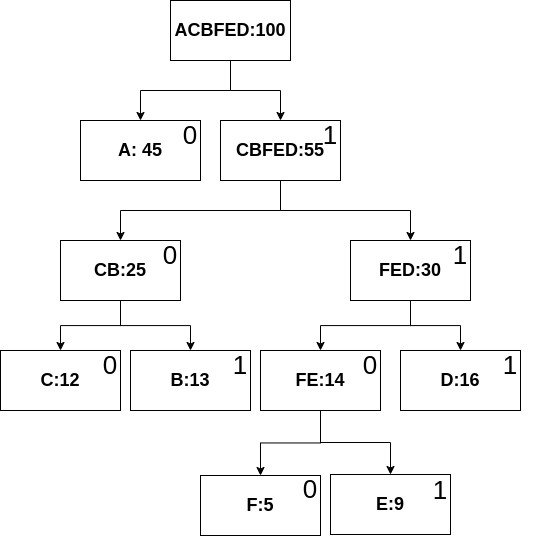
\includegraphics[scale=0.5]{Huffman.png}
        \end{center}

      \item Tentukan kode Huffman untuk setiap simbol.
        \begin{center}
          \begin{adjustbox}{scale=1,center}
            \begin{tabular}{ |c|c| } 
              \hline
              Simbol & Frekuensi Kemunculan \\ \hline
              A & 0  \\ \hline
              B & 101  \\ \hline
              C & 100 \\ \hline
              D & 111 \\ \hline
              E & 1101 \\ \hline
              F & 1100 \\ \hline
            \end{tabular}
          \end{adjustbox}
        \end{center}

    \end{enumerate}

  \item Sebuah platform live streaming akan menayangkan 30 video secara bersamaan, dengan
    spesifikasi berikut:

    \begin{itemize}
      \item Bitrate per video: 4 Mbps
      \item Durasi setiap video: 15 menit
      \item Jumlah Penonton: 150.000 penonton menonton secara bersamaan setiap detiknya.
      \item Ukuran Buffer: 20 MB
      \item Kecepatan Transfer Data: 200 Mbps
      \item Waktu Pengkodean Server: 0.7 detik
      \item Waktu Transmisi Jaringan: 1.2 detik
      \item Waktu Dekoding & Pemutaran Klien: 0.8 detik
    \end{itemize}

    Pertanyaan:
    \begin{enumerate}
      \item Hitung Total Bandwidth yang diperlukan.

        \[
          Total\ Bandwith\ =\ Bitrate\ X\ Jumlah\ Pengguna 
        \]

        \[
          Total\ Bandwith\ =\  4\ Mbps\ X\ 150.000\ =\ 600.000\ Mbps 
        \]

      \item Hitung waktu buffering minimal yang diperlukan untuk mulai memutar video.
        \[
          Waktu\ Buffering(detik)\ = \frac{Ukuran\ Buffer(bit)}{Kecepatan\ Transfer\ Data(bps)}
        \]

        \[
          Ukuran\ Buffer(bit)\ =\ 20\ X\ 8.000.000\ =\ 160.000.000\ bit
        \]

        \[
          Kecepatan\ Transfer(bit)\ =\ 200\ X\ 1.000.000\ =\ 200.000.000\ bps
        \]

        \[
          Waktu\ Buffering(detik)\ = \frac{160.000.000}{200.000.000} = 0.8\ detik
        \]

      \item Hitung waktu tunda total (end-to-end delay) dari server ke klien.
        \[
          Latency\ Total\ =\ 0.7\ detik\ +\ 1.2\ detik\ +\ 0.8\ detik\ =\ 2.7\ detik
        \]

      \item Hitung total kapasitas penyimpanan yang diperlukan untuk menyimpan semua
        video selama 15 menit penuh. 
        \[
          Bitrate\ Video(bps)\ =\ 4\ Mbps\ =\ 4.000.000\ bps
        \]

        \[
          Durasi\ Video(detik)\ =\ 15\ menit\ X\ 60\ =\ 900\ detik
        \]

        \[
          Ukuran\ File\ Per\ Video(bps)\ =\ 4.000.000\ bps\ X\ 900\ =\ 3.600.000.000
        \]

        \[
          Ukuran\ File\ Per\ Video(byte)\ =\ \frac{3.600.000.000}{8} = 450.000.000\ byte
        \]

        \[
          Ukuran\ File\ Per\ Video(GB)\ =\ \frac{450.000.000}{1.000.000.000} = 0.45\ GB
        \]

        \[
          Total\ Penyimpanan\ =\ 0.45\ GB\ X\ 30\ =\ 13.5\ GB
        \]


    \end{enumerate}
  \end{enumerate}
\end{document}
